\documentclass[a4paper,14pt]{article}
\usepackage{xcolor}
\usepackage{amsmath,amsfonts,amssymb}
\usepackage{geometry}
\usepackage{fancyhdr}
\usepackage{graphicx}
\usepackage{titlesec}
\usepackage{tikz}
\usepackage{booktabs}
\usepackage{array}
\usetikzlibrary{shadows}
\usepackage{tcolorbox}
\usepackage{float}
\usepackage{lipsum}
\usepackage{mdframed}
\usepackage{pagecolor}
\usepackage{mathpazo}   % Palatino font (serif)
\usepackage{microtype}  % Better typography

\setlength{\parindent}{0pt}

% Page background color
\pagecolor{gray!10!white}

% Geometry settings
\geometry{margin=0.5in}
\pagestyle{fancy}
\fancyhf{}

% Fancy header and footer
\fancyhead[C]{\textbf{\color{blue!80}CS663 Assignment-4}}
% \fancyhead[R]{\color{blue!80}Saksham Rathi}
\fancyfoot[C]{\thepage}

% Custom Section Color and Format with Sans-serif font
\titleformat{\section}
{\sffamily\color{purple!90!black}\normalfont\Large\bfseries}
{\thesection}{1em}{}

% Custom subsection format
\titleformat{\subsection}
{\sffamily\color{cyan!80!black}\normalfont\large\bfseries}
{\thesubsection}{1em}{}

% Stylish Title with TikZ (Enhanced with gradient)
\newcommand{\cooltitle}[1]{%
  \begin{tikzpicture}
    \node[fill=blue!20,rounded corners=10pt,inner sep=12pt, drop shadow, top color=blue!50, bottom color=blue!30] (box)
    {\Huge \bfseries \color{black} #1};
  \end{tikzpicture}
}
\usepackage{float} % Add this package

\newenvironment{solution}[2][]{%
    \begin{mdframed}[linecolor=blue!70!black, linewidth=2pt, roundcorner=10pt, backgroundcolor=yellow!10!white, skipabove=12pt, skipbelow=12pt]%
        \textbf{\large #2}
        \par\noindent\rule{\textwidth}{0.4pt}
}{
    \end{mdframed}
}

% Document title
\title{\cooltitle{CS663 Assignment-4}}
\author{{\bf Saksham Rathi, Kavya Gupta, Shravan Srinivasa Raghavan} \\
\small Department of Computer Science, \\
Indian Institute of Technology Bombay \\}
\date{}

\begin{document}
\maketitle

\section*{Question 4}

\begin{solution}{Solution}
	Note: All values of Recognition Rate in the plots are in fractions.
	\begin{itemize}
		\item \textbf{ORL Database:}

		Code is in \texttt{myMainScript\_ORL.m}.

		Plots for Recognition Rate vs $k$ for the following methods are given below:-

		\begin{itemize}
			\item Using \texttt{eig} function
			
			\begin{center}
				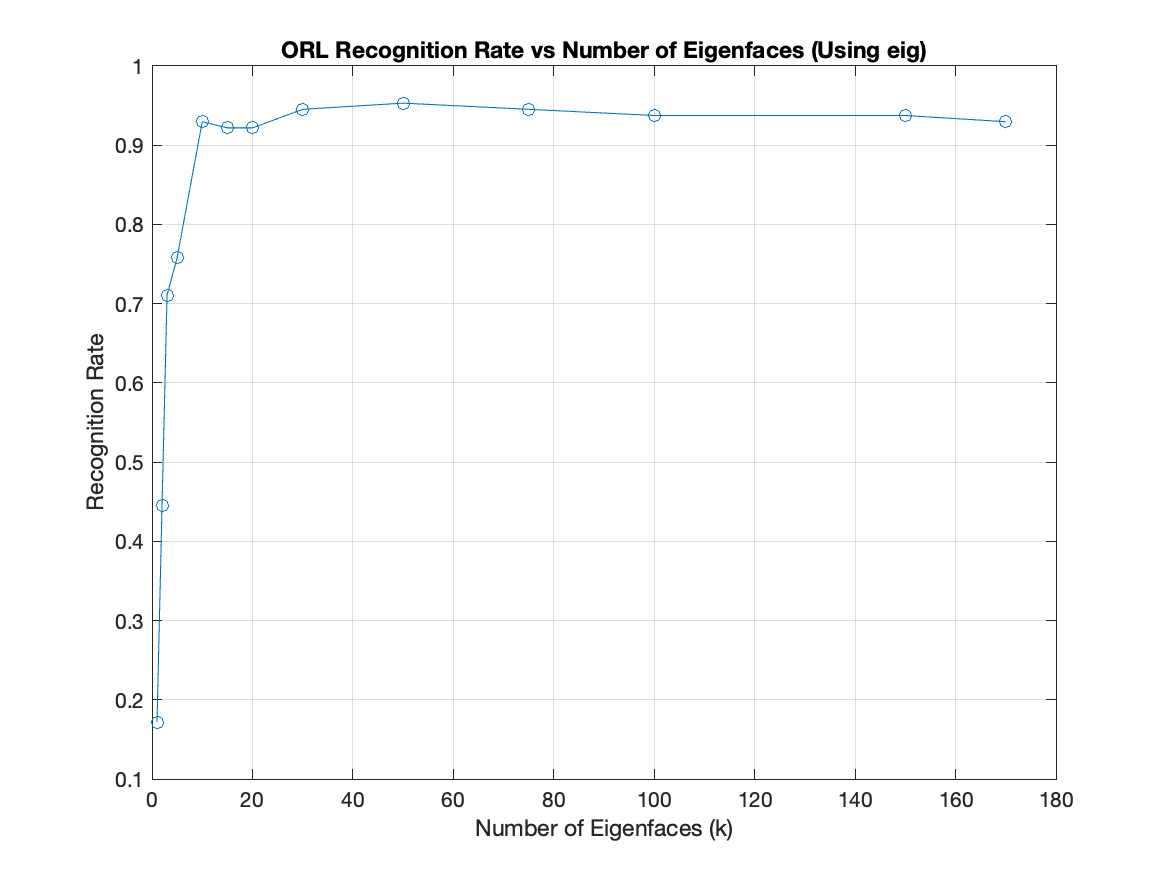
\includegraphics[scale=0.4]{../images/ORL_eig.png}
			\end{center}

			\item Using \texttt{svd} function
			
			\begin{center}
				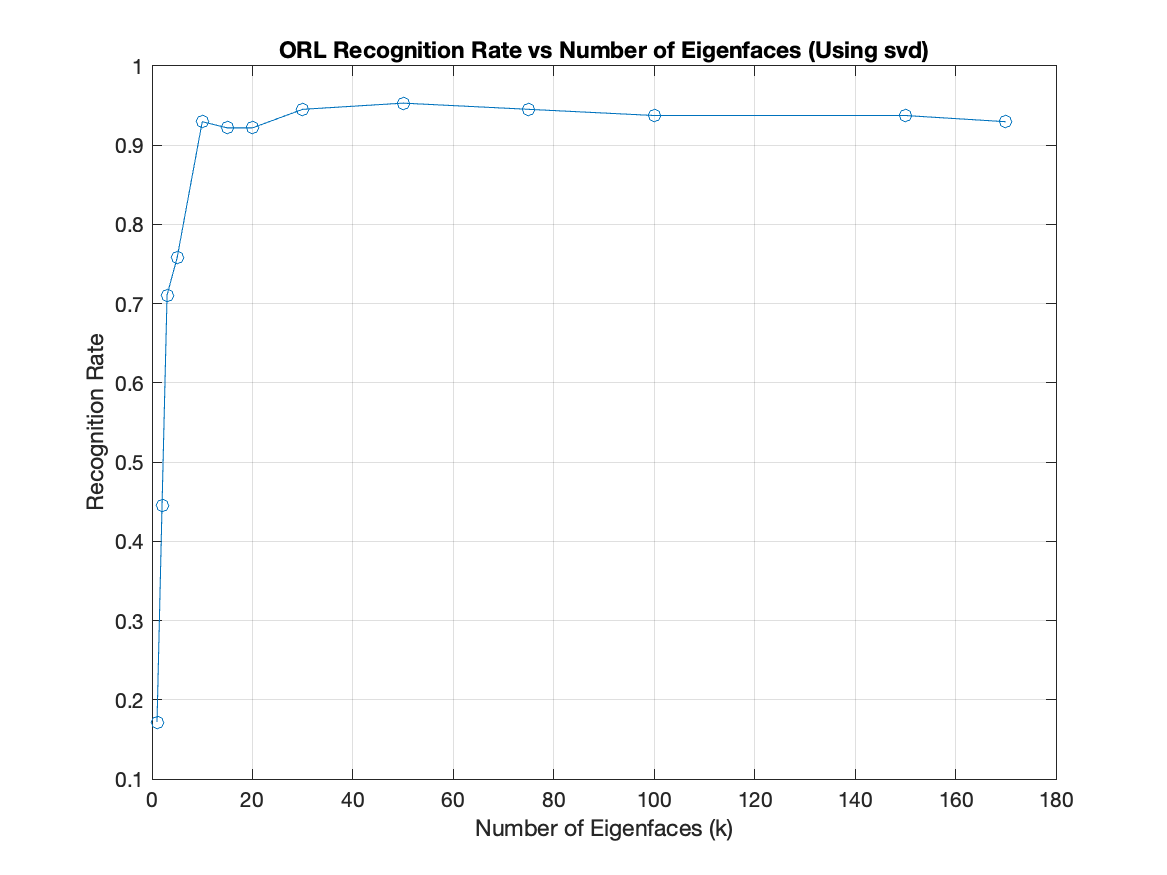
\includegraphics[scale=0.4]{../images/ORL_svd.png}
			\end{center}
		\end{itemize}

		We can see that both are looking same.\ Maximum Recognition Rate is around $0.953$ for $k = 50$ (in both cases).

		\item \textbf{Yale Database:}

		Code is in \texttt{myMainScript\_Yale.m}.\ As asked by the question, \texttt{eig} function has been used.

		Plots for Recognition Rate vs $k$ for the following parts are given below:-

		\begin{itemize}
			\item Part (a)

			\begin{center}
				\includegraphics[scale=0.4]{../images/Yale\_a.png}
			\end{center}

			Maximum Recognition Rate is around $0.356$ for $k = 1000$.

			\item Part (b)

			\begin{center}
				\includegraphics[scale=0.4]{../images/Yale\_b.png}
			\end{center}

			Maximum Recognition Rate is around $0.606$ for $k = 1000$.
		\end{itemize}

		It seems that the results were better once the eigen-coefficients related to the three largest eigenvalues were dropped.

		\item \textbf{Reconstruction:}
		
		Code is in \texttt{myMainScript\_reconstruction.m}.\ We used the \texttt{svd} function for reconstruction of the image.\ For example here, we chose the very first image of the first person.

		\begin{center}
			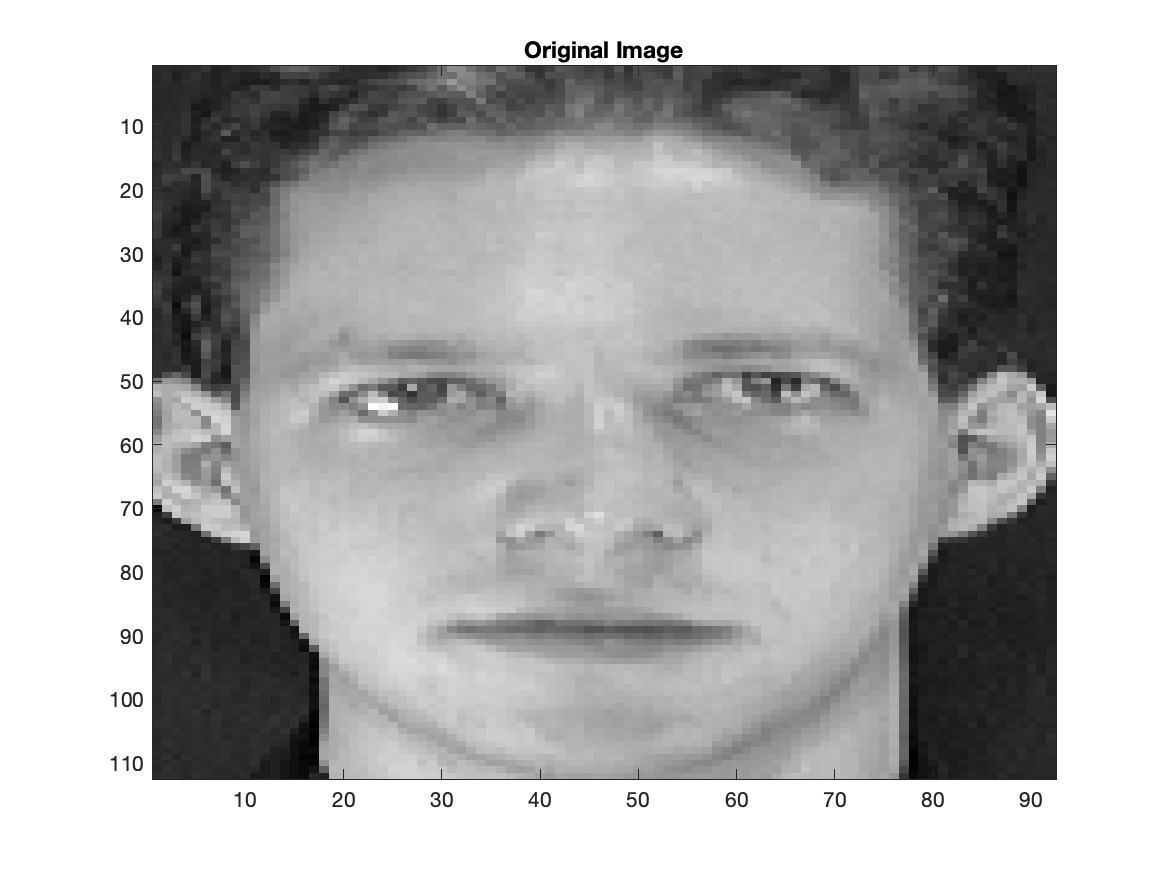
\includegraphics[scale=0.21]{../images/original_image.png}
		\end{center}

		Reconstructed images for different values of $k$ are:-

		\begin{center}
			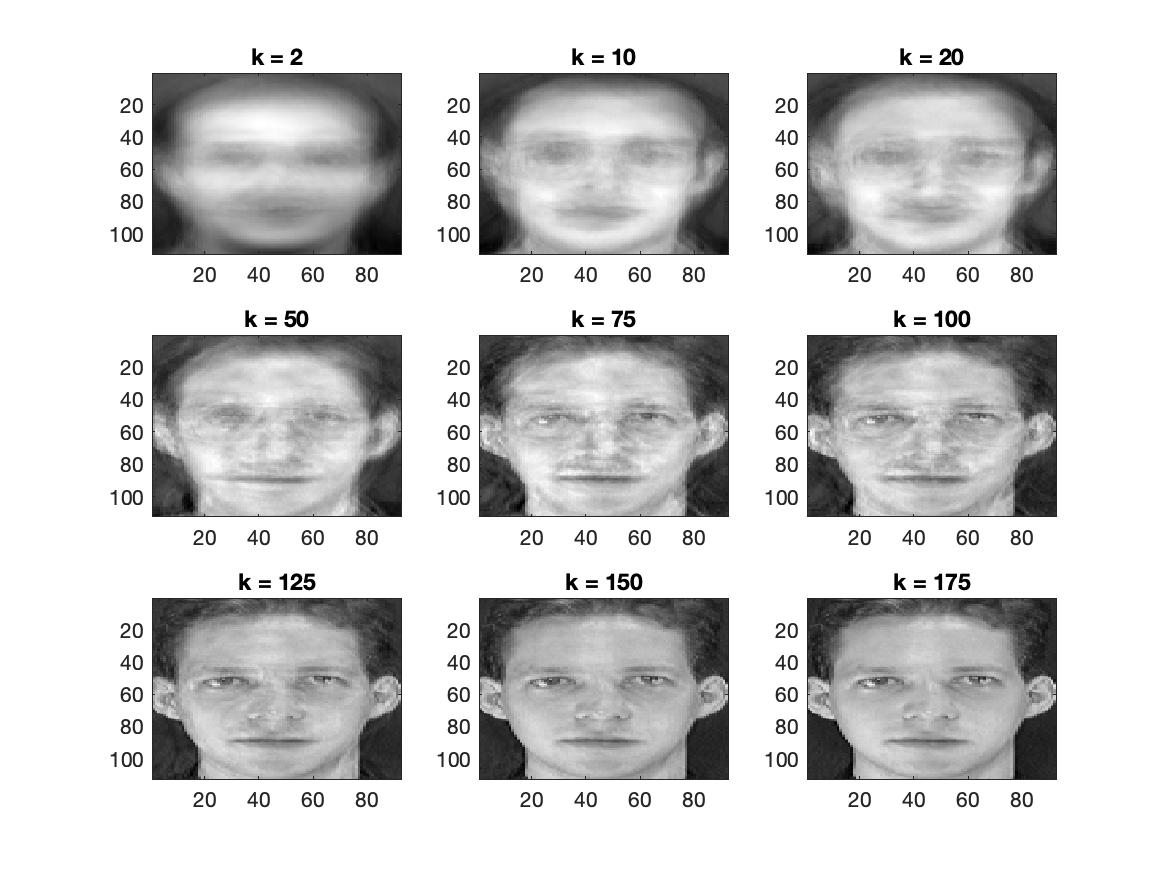
\includegraphics[width=0.9\linewidth]{../images/ORL_reconstructed_faces.png}
		\end{center}

		The $25$ eigenvectors (eigenfaces) corresponding to the $25$ largest eigenvalues are:-

		\begin{center}
			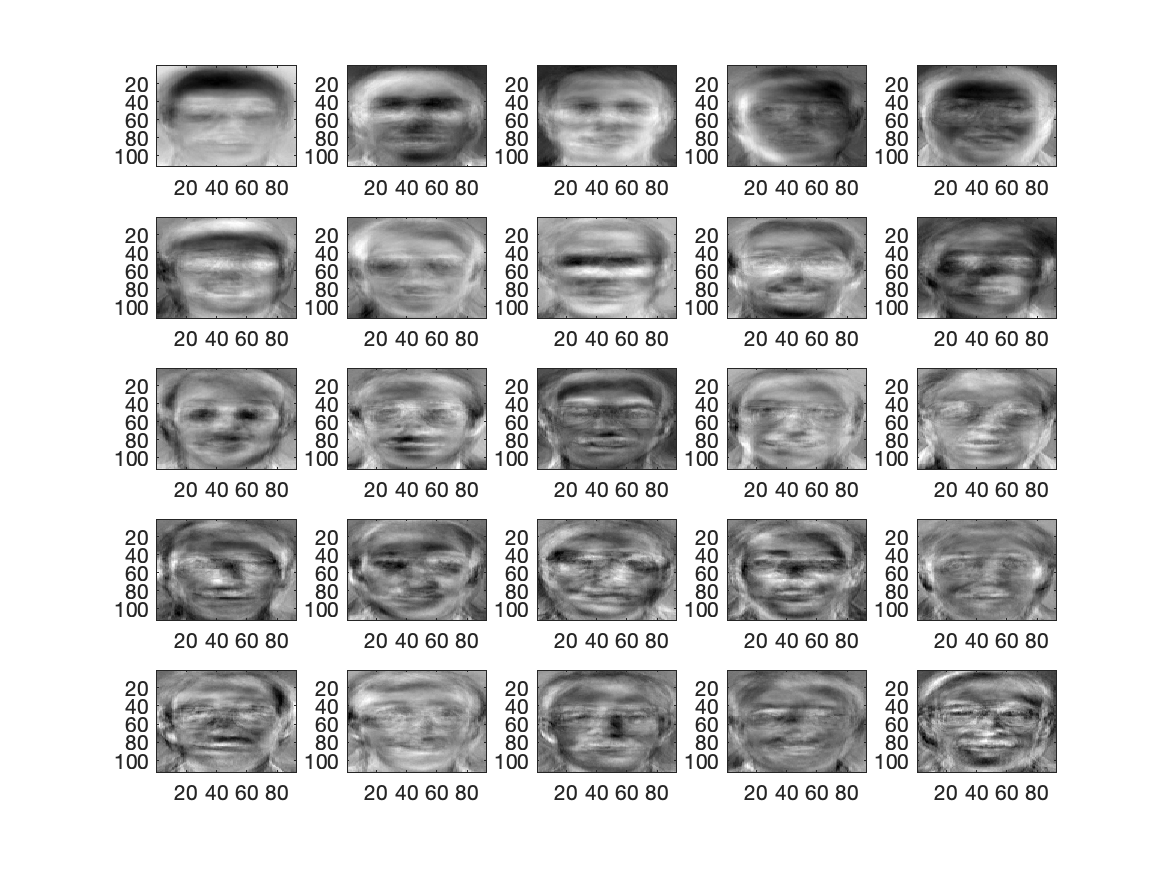
\includegraphics[width=0.88\linewidth]{../images/ORL_eigenfaces.png}
		\end{center}

		The top leftmost corresponds to the largest eigenvalue, the one to its right is second largest and so on.
	\end{itemize}
\end{solution}

\end{document}